\chapter{Test Environment} 
\label{chap:3}
This chapter contains information about the test environment used in next chapters including description of benchmarking method and specification of hardware and software used in experiments. These parameters would be required if one set out to reproduce the collected data or to compare experiments conducted on different hardware or software.

\section{Benchmarking}
Tests performed in this paper will be constructed and executed using .NET benchmarking tool, \emph{BenchmarkDotNet}. It is an open source library which helps in transforming methods into benchmarks and producing reproducible experiments. The results are guaranteed to be reliable and precise by the usage of \emph{perfolizer} statistical engine. 

The tool is well equiped for the topic of this paper. It measures performance as mean estimated time, removes outlier data, calculates error ranges and standard deviation. Additionaly, \emph{MemoryDiagnoser} tracks GC generations and memory allocations which is important when testing parallel programs. Listing~\ref{lst:QSBenchClass} showcases one of the benchmarks which will be used during the experiments.
These benchmarks were developed with the use of \emph{Pro .NET benchmarking: the art of performance measurement} by Andrey Akinshin~\cite{Akinshin2019}.

\begin{lstlisting}[language={[sharp]c}, style=sharpcstyle, caption={Quicksort benchmark class}, label={lst:QSBenchClass}]
namespace Net47Benchmarking
{
  [SimpleJob(RuntimeMoniker.Net472)]
  [SimpleJob(RuntimeMoniker.NetCoreApp31)]
  [MemoryDiagnoser]
  [RPlotExporter]
  [CsvMeasurementsExporter]
  public class Net47QuickSortBenchmark
  {
    private readonly SequentialImperativeQuickSort _sequentialImperativeQuickSort = new SequentialImperativeQuickSort();
    private readonly ParallelImperativeQuickSort _parallelImperativeQuickSort = new ParallelImperativeQuickSort();
    private readonly OptimizedParallelImperativeQuickSort _optimizedParallelImperativeQuickSort =
      new OptimizedParallelImperativeQuickSort((int)Math.Log(Environment.ProcessorCount, 2) + 4);

    private readonly SequentialFunctionalQuickSort _sequentialFunctionalQuickSort = new SequentialFunctionalQuickSort();
    private readonly ParallelFunctionalQuickSort _parallelFunctionalQuickSort = new ParallelFunctionalQuickSort();
    private readonly OptimizedParallelFunctionalQuickSort _optimizedParallelFunctionalQuickSort =
      new OptimizedParallelFunctionalQuickSort((int)Math.Log(Environment.ProcessorCount, 2) + 4);

    // ReSharper disable once MemberCanBePrivate.Global
    public int[] Data;

    // ReSharper disable once MemberCanBePrivate.Global
    [Params(10000, 100000, 1000000, 10000000)] public int N;

    [GlobalSetup]
    public void Setup()
    {
      var random = new Random(42);

      Data = Enumerable
        .Range(0, N)
        .Select(_ => random.Next())
        .ToArray();
    }


    [Benchmark]
    public ImmutableList<int> SequentialFunctionalQuickSort()
       => _sequentialFunctionalQuickSort.Sort(Data).Result;

    [Benchmark]
    public ImmutableList<int> ParallelFunctionalQuickSort()
      => _parallelFunctionalQuickSort.Sort(Data).Result;

    [Benchmark]
    public ImmutableList<int> OptimizedParallelFunctionalQuickSort()
      => _optimizedParallelFunctionalQuickSort.Sort(Data).Result;

    [Benchmark]
    public ImmutableList<int> SequentialImperativeQuickSort()
      => _sequentialImperativeQuickSort.Sort(Data).Result;

    [Benchmark]
    public ImmutableList<int> ParallelImperativeQuickSort()
      => _parallelImperativeQuickSort.Sort(Data).Result;

    [Benchmark]
    public ImmutableList<int> OptimizedParallelImperativeQuickSort()
      => _optimizedParallelImperativeQuickSort.Sort(Data).Result;
  }
}
\end{lstlisting}


\clearpage
\section{Hardware and software} 
Each machine is different in it's own way, it is imperative to use the same hardware for all experiments to accurately benchmark tested software. Thus one cannot expect to receive the same results when conducting testing as presented later on this paper but in different settings. Specification of the machine used for development and benchmarking is presented in tab.~\ref{tab:HardSpec}. It's a middle-range (for 2021) machine for personal use.
\begin{table}[!ht]
    \centering
    \caption{Machine specification}
		\label{tab:HardSpec}
    \begin{tabular}{ll}
			\toprule
			CPU  & AMD Ryzen 5 3600 3.95 GHz 6 Cores 12 Logical Processors \\
			RAM  & Patriot 16GB 3000MHz CL16 \\ 
			MB   & Asus Prime X470 - Pro \\ 
			Disk & Samsung SSD 970 EVO Plus \\
			GPU  & AMD Radeon RX 5700 XT \\ 
			OS   & Windows 10 x64 Pro Build 19042 \\ 
			BIOS & American Megatrends 5406 \\ 
			\bottomrule
    \end{tabular}
\end{table}

AMD Ryzen 5 3600 is built using Zen2 architecture,  the successor of AMD's Zen and Zen+ microarchitectures. From the most notable features it enables 2 threads per physical core (SMT) and optimized processor caches: L1 cache with 32 kB  per core and 8-way associative input and output, L2 with 512 kB per core and L3 cache with 16MB per core. Fig.~\ref{fig:Zen} showcases microarchitecutre overview of Zen2 processors~\cite{Zen}.

\begin{figure}[!ht]
	\centering
		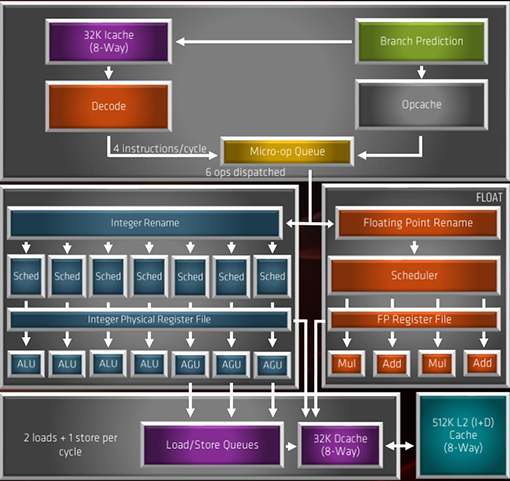
\includegraphics[width = 0.7\textwidth]{figures03/Zen.PNG}
	\caption{Zen2 microarchitecture}
	\label{fig:Zen}
\end{figure}

The aforementioned caches function as memory banks between main memory and the CPU. They store operation instructions and frequently used memory locations. The caches are usualy divided into three levels which are checked for hits in a top down manner:
\begin{itemize}
	\item \textbf{L1 cache} is the smallest, but the fastest cache. In case of Zen2 architecture it actually consists of two equal size caches, one for program data, second one for instructions. 
	\item \textbf{L2 cache} is next in line, it serves the same function as L1 but it is slightly bigger and slightly  slower.
	\item \textbf{L3 cache} is significantly bigger but accesing it will have  greater impact on performance. In Zen2 architecture this cache is shared between cores in one chiplet.  
\end{itemize}

Size and latency of the caches is presented on fig.~\ref{fig:Cache}.

\begin{figure}[!ht]
	\centering
		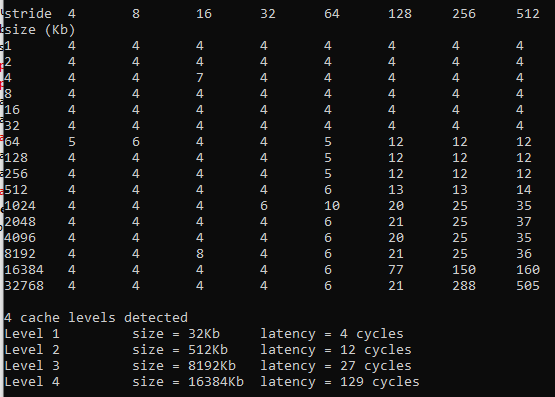
\includegraphics[width = 0.7\textwidth]{figures03/Cache.PNG}
	\caption{Ryzen 5 3600 cache sizes and latency}
	\label{fig:Cache}
\end{figure}

This chapter described how benchmarks will be conducted and specified hardware and software used in testing. Chapter that follows will introduce algorithms and software used in testing and their multiple implementations using parallel techniques. 
